\documentclass[../doc.tex]{subfiles}
\begin{document}

\subsection{Mediante inducción estructural defina la estructura del grafo.}

Debemos definir un grafo de a través de la inducción estructural, con base en
las instrucciones se usará una lista de adyacencia, por lo tanto, lo primero
que debemos crear es una lista de números para que posteriormente el grafo sea
una lista de listas de números. Se define la lista y algunas funciones útiles.

\subsubsection*{\emph{Lista de naturales}}
\textbf{Definición:}
\[ \emptyset \in \mathcal{L}_{\mathbb{N}} \]
\[ L \in \mathcal{L}_\mathbb{N} \Rightarrow L \rightarrow k \in \mathcal{L}_\mathbb{N}, \forall k \in \mathbb{N}\]
\textbf{Operaciones:}
\[ Insertar(L, k) = L \rightarrow k\]
\newline
\textbf{Ejemplos:}

\[ \rightarrow 0 \rightarrow 2 \rightarrow 7 \]
\[ Insertar(\rightarrow 0 \rightarrow 2 \rightarrow 7, 10) =  \rightarrow 0 \rightarrow 2 \rightarrow 7 \rightarrow 10\]
\[ Insertar(\emptyset, 4) = \rightarrow 4 \]

\subsubsection*{\emph{Definición del grafo}}
Ahora se crea el grafo utilizando la lista, es importante notar que la
definición de este grafo, es la implementación de un grafo direccional, las
listas de adyacencia por lo general son para grafos dirigidos. Haremos que sea
un grafo no dirigido posteriormente con el método de $InsertarNodo$, ya que,
ese método creara una conexión de i a j y de j a i, manteniendo las propiedades
de un grafo no dirigido \footnote{A excepción de que en este grafo la cantidad
flechas será el doble que la cantidad de aristas reales en el grafo.}. Se
utilizará una flecha diferente a la de la lista para distinguirlas.

\emph{Definición}

\[ \emptyset \in \mathcal{G} \]
\[ G \in \mathcal{G} \Rightarrow (L) \rightarrowtail G \in \mathcal{G} , \forall L \in \mathcal{L}_\mathbb{N} \]

Ejemplos:

\[ ( \rightarrow 2 \rightarrow 3) \rightarrowtail (\rightarrow 3) \rightarrowtail (\rightarrow 0) \rightarrowtail (\rightarrow 0 \rightarrow 1) \rightarrowtail \emptyset \]
Representa el siguiente grafo: 

\begin{center}
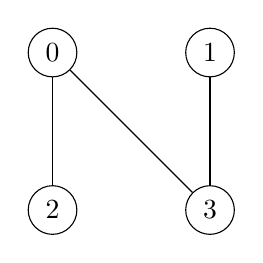
\begin{tikzpicture}
  % Nodos
  \node[circle, draw] (0) at (0,0) {0};
  \node[circle, draw] (1) at (2,0) {1};
  \node[circle, draw] (2) at (0,-2) {2};
  \node[circle, draw] (3) at (2,-2) {3};
  
  % Aristas
  \draw (0) -- (2);
  \draw (0) -- (3);
  \draw (1) -- (3);
\end{tikzpicture}
\end{center}

\subsection{Insertar Nodo}
Esta parte se complica un poco, al ser un grafo no dirigido, ya que, no se
puede solo añadir la lista al final del grafo que ya tenemos, porque se crearía
asimetría en los datos del grafo, es decir, se puede llegar de j a i, pero no
de i a j.

Por lo tanto, lo que debemos hacer es añadir la lista al final, pero además
debemos agregar en cada lista del grafo que corresponda, un borde a la nueva
arista.

Para hacer esto lo primero que haré es una función que conecte el nodo i y j de
un grafo G.

\[ Conectar((L) \rightarrowtail G, 0, j) = (Insertar(L, j)) \rightarrowtail G \]
\[ Conectar((L) \rightarrowtail G, i, j) = (L) \rightarrowtail Conectar(G, i-1, j) \]

Además, ahora sería útil una función que conecte una lista de nodos a un nodo,
para utilizarla en la función final.

\[ ConectarTodos(G, \emptyset, j) = G  \]
\[ ConectarTodos(G, i \rightarrow L, j) = ConectarTodos(Conectar(G, i, j), L, j)  \]

Ahora que ya podemos conectar el nodo i con el j, necesitamos saber qué valor 
tendrá j, por lo tanto, tenemos que saber cuantos nodos hay en el grafo para 
conocer cuál será el valor del siguiente.

\[ ContarNodos(\emptyset) = 0 \]
\[ ContarNodos((L) \rightarrowtail G) = 1 + ContarNodos(G) \]

Con estas funciones auxiliares creadas, el trabajo se facilita mucho y ya 
podemos definir la función InsertarNodo.

\[ InsertarNodo(G, L) = ConectarTodos(G \rightarrowtail (L), L, ContarNodos(G)) \]

\subsection{Cantidad mínima de aristas}

Debemos demostrar $ a_n = n - 1 $ donde $ a_n $ es la mínima cantidad de aristas
necesarias para conectar n nodos.

\subsubsection*{\emph{B.I.}}
\[ n = 1 \]

\begin{center}
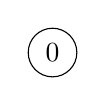
\begin{tikzpicture}
  % Nodos
  \node[circle, draw] (0) at (0,0) {0};
\end{tikzpicture}
\end{center}
En este caso hay 0 aristas, lo que concuerda con $a_1 = 1 - 1 = 0$. :)

\[ n = 2 \]

\begin{center}
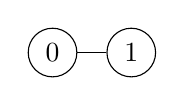
\begin{tikzpicture}
  % Nodos
  \node[circle, draw] (0) {0};
  \node[circle, draw] (1) [right of=0] {1};

  \draw (0) -- (1);
\end{tikzpicture}
\end{center}
En este caso hay 1 arista, lo que concuerda con $a_2 = 2 - 1 = 1$. :)


\[ n = 5 \]

\begin{center}
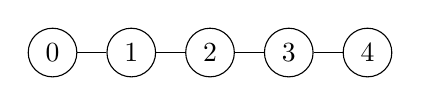
\begin{tikzpicture}
  % Nodos
  \node[circle, draw] (0) {0};
  \node[circle, draw] (1) [right of=0] {1};
  \node[circle, draw] (2) [right of=1] {2};
  \node[circle, draw] (3) [right of=2] {3};
  \node[circle, draw] (4) [right of=3] {4};

  \draw (0) -- (1);
  \draw (2) -- (1);
  \draw (2) -- (3);
  \draw (4) -- (3);
\end{tikzpicture}
\end{center}
En este caso hay 4 aristas, lo que concuerda con $a_5 = 5 - 1 = 4$. :)

\subsubsection*{\emph{H.I.}}
Ahora vamos asumir que $ a_n = n - 1 $.

\subsubsection*{\emph{T.I.}}
PDQ: $a_{n+1} = (n + 1) -1 = n$ \\
Partimos de un grafo que ya estaba mínimamente conectado, y queremos añadir un
nodo. Tenemos que añadirlo con la mínima cantidad de aristas posibles, esto se
hace conectándolo con cualquier nodo que estuviese originalmente en el grafo,
ya que así solo añadimos 1 arista, lo cual es mínimo. Cuando hayamos hecho
esto, el número total de aristas se habrá incrementado en 1 al igual que lo
hará la cantidad nodos, con relación al grafo inicial.

\[\therefore a_{n+1} = a_{n} + 1\]
Por H.I
\[a_{n+1} = (n - 1) + 1\]
\[a_{n+1} = n\]
 

\subsection{Cantidad máxima de aristas}
Debemos demostrar $a_n = \frac{n(n-1)}{2} $ donde $a_n$ es la máxima cantidad de 
aristas que podemos utilizar para conectar n nodos.

\subsubsection*{\emph{B.I}}
\[ n = 1 \]

\begin{center}
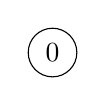
\begin{tikzpicture}
  % Nodos
  \node[circle, draw] (0) at (0,0) {0};
\end{tikzpicture}
\end{center}
En este caso hay 0 aristas, lo que concuerda con $a_1 = \frac{1(1-1)}{2} = 0$. :)

\[ n = 2 \]

\begin{center}
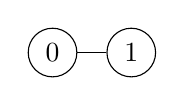
\begin{tikzpicture}
  % Nodos
  \node[circle, draw] (0) {0};
  \node[circle, draw] (1) [right of=0] {1};

  \draw (0) -- (1);
\end{tikzpicture}
\end{center}
En este caso hay 1 arista, lo que concuerda con $a_2 = \frac{2(2-1)}{2} = 1$. :)


\[ n = 5 \]

\begin{center}
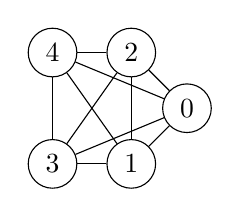
\begin{tikzpicture}
  % Nodos
  \node[circle, draw] (0) {0};
  \node[circle, draw] (1) [below left of=0] {1};
  \node[circle, draw] (2) [above left of=0] {2};
  \node[circle, draw] (3) [left of=1] {3};
  \node[circle, draw] (4) [left of=2] {4};

  \draw (0) -- (1);
  \draw (0) -- (2);
  \draw (0) -- (3);
  \draw (0) -- (4);
  \draw (1) -- (2);
  \draw (1) -- (3);
  \draw (1) -- (4);
  \draw (2) -- (3);
  \draw (2) -- (4);
  \draw (3) -- (4);
\end{tikzpicture}
\end{center}
En este caso hay 10 aristas, lo que concuerda con $a_5 = \frac{5(5-1)}{2}$ = 10. :)

\[ n = 6 \]

\begin{center}
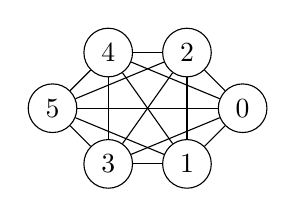
\begin{tikzpicture}
  % Nodos
  \node[circle, draw] (0) {0};
  \node[circle, draw] (1) [below left of=0] {1};
  \node[circle, draw] (2) [above left of=0] {2};
  \node[circle, draw] (3) [left of=1] {3};
  \node[circle, draw] (4) [left of=2] {4};
  \node[circle, draw] (5) [below left of=4] {5};

  \draw (0) -- (1);
  \draw (0) -- (2);
  \draw (0) -- (3);
  \draw (0) -- (4);
  \draw (1) -- (2);
  \draw (1) -- (3);
  \draw (1) -- (4);
  \draw (2) -- (3);
  \draw (2) -- (4);
  \draw (3) -- (4);
  \draw (5) -- (0);
  \draw (5) -- (1);
  \draw (5) -- (2);
  \draw (5) -- (3);
  \draw (5) -- (4);
\end{tikzpicture}
\end{center}
En este caso hay 15 aristas, lo que concuerda con $a_6 = \frac{6(6-1)}{2} = 15$. :)


\subsubsection*{\emph{H.I}}
Ahora asumiremos correcto que:
\[ a_n = \frac{n(n-1)}{2} \]

\subsubsection*{\emph{T.I}}
\emph{PDQ:}
\[ a_{n+1} = \frac{(n+1)((n+1) - 1)}{2} = \frac{(n+1)n}{2} \]
Si tenemos un grafo que está máximamente conectado con n nodos y queremos
añadir uno nuevo, podemos añadir como máximo n aristas, ya que, será añadida
una conexión a cada nodo que ya estaba en el grafo, no podemos añadir más
debido todas las otras ya están en el grafo por estar máximamente conectado.
\[ \therefore a_{n+1} = a_n + n \]
\emph{Por H.I.}
\[ a_{n+1} = \frac{(n-1)n}{2} + n = \frac{(n-1)n + 2n}{2} = \frac{n(n-1+2)}{2} = \frac{(n+1)n}{2} \]

\end{document}
